\documentclass[11pt]{article}
\usepackage[T1]{fontenc}
\usepackage{lmodern}
\usepackage[margin=1.05in]{geometry}
\usepackage{amsmath,amssymb,amsthm,mathtools}
\usepackage{microtype}
\usepackage{xcolor}
\usepackage{tikz}
\usepackage[colorlinks=true,linkcolor=blue!45!black,citecolor=blue!45!black,urlcolor=blue!45!black]{hyperref}
\usepackage{bookmark}
\usepackage[numbers,sort&compress]{natbib}
\pdftrailerid{}
\hypersetup{pdftitle={A nonspectrahedral hyperbolicity cone},pdfauthor={OpenAI}}
\newcommand{\R}{\mathbb R}
\newcommand{\Sym}{\mathbb S}
\newcommand{\norm}[1]{\left\lVert#1\right\rVert}
\newcommand{\op}{\mathrm{op}}
\DeclareMathOperator{\adj}{adj}
\DeclareMathOperator{\tr}{tr}
\DeclareMathOperator{\proj}{proj}
\newtheorem{theorem}{Theorem}[section]
\newtheorem{proposition}[theorem]{Proposition}
\newtheorem{lemma}[theorem]{Lemma}
\newtheorem{corollary}[theorem]{Corollary}
\theoremstyle{remark}
\newtheorem{remark}[theorem]{Remark}
\numberwithin{equation}{section}
\setlength{\emergencystretch}{1.5em}
\title{A nonspectrahedral hyperbolicity cone}
\author{OpenAI}
\date{September 24, 2026}
\begin{document}
\maketitle
\begin{abstract}
We construct a homogeneous polynomial of degree $16$ in $23$ real variables
whose hyperbolicity cone has no representation by a finite homogeneous
real symmetric linear matrix inequality. This disproves the geometric Generalized Lax
conjecture.
\end{abstract}
\tableofcontents
\section{Introduction}
\label{sec:introduction}

A homogeneous polynomial $p\in\R[x_1,\ldots,x_m]$ of degree $d\geq1$ is
\emph{hyperbolic with respect to} $e\in\R^m$ if $p(e)\ne0$ and every root of
$t\mapsto p(te-x)$ is real for every $x\in\R^m$.
Write these roots, with multiplicity, as $\lambda_1(x),\ldots,\lambda_d(x)$.
The closed hyperbolicity cone is
\[
 \Lambda_+(p,e)=\{x\in\R^m:\lambda_j(x)\geq0\text{ for }1\leq j\leq d\}.
\]
We write $\Sym^N$ for the real symmetric $N\times N$ matrices and
$A\succeq0$ (respectively, $A\succ0$) for positive semidefiniteness
(respectively, positive definiteness).
A cone is \emph{spectrahedral} if it has the form
\begin{equation}
 K=\{x\in\R^m:L(x)\succeq0\},\qquad
 L(x)=\sum_{i=1}^m x_iA_i,\quad A_i\in\Sym^N,
 \label{eq:spectrahedral}
\end{equation}
for some finite $N\geq1$.
The geometric Generalized Lax conjecture asserts that every hyperbolicity
cone is spectrahedral. We give a counterexample.

\subsection{The explicit polynomial}

All indices in $\{1,2,3\}$ in the following construction are cyclic.
For $z,y\in\R^3$, let
\begin{equation}
 b(z,y)=\sum_{i=1}^3 z_i^2y_i^2
       -2\sum_{1\leq i<j\leq3}z_iy_iz_jy_j
       +\sum_{i=1}^3z_i^2y_{i+1}^2.
 \label{eq:form}
\end{equation}
This is the coefficient-one Choi--Lam biquadratic
form~\cite[Section~4]{choi-lam-1977}.
Define $Q(y)\in\Sym^3$ by
\[
 Q(y)_{ii}=y_i^2+y_{i+1}^2,\qquad
 Q(y)_{ij}=-y_iy_j\quad(i\ne j),
\]
so that $b(z,y)=z^\top Q(y)z$.
For $a\in\R$, $r\in\R^3$ and $T\in\Sym^3$, define the linear map
$\Phi_y:\Sym^4\to\Sym^4$ by
\begin{equation}
 \Phi_y\!\begin{pmatrix}a&r^\top\\r&T\end{pmatrix}
 =\begin{pmatrix}
    \tr(Q(y)T)&-r^\top Q(y)\\
    -Q(y)r&aQ(y)
   \end{pmatrix}.
 \label{eq:phi}
\end{equation}
The dependence on $y$ is homogeneous quadratic. If $\adj X$ denotes the
adjugate of $X$, set
\begin{equation}
 p(X,Z,y)=\det\big((\det X)Z-\Phi_y(\adj X)\big),
 \qquad (X,Z,y)\in\Sym^4\times\Sym^4\times\R^3.
 \label{eq:polynomial}
\end{equation}
This formula is polynomial even when $X$ is singular. The ambient space
has dimension $10+10+3=23$.

\begin{theorem}\label{thm:main}
The polynomial \eqref{eq:polynomial} is homogeneous of degree $20$ and
hyperbolic with respect to $e=(I_4,I_4,0)$, with $p(e)=1$.
Its closed hyperbolicity cone $K=\Lambda_+(p,e)$ is not spectrahedral:
for every finite $N\geq1$ and every real linear map
$L:\Sym^4\times\Sym^4\times\R^3\to\Sym^N$,
\[
 K\ne\{(X,Z,y):L(X,Z,y)\succeq0\}.
\]
\end{theorem}

The conclusion concerns the cone itself, so it allows every possible
defining pencil and every finite matrix size. The compact formula for $p$
is convenient for the proof, but one determinant factor can be removed.

\begin{corollary}\label{cor:reduced}
The quotient $q=p/\det X$ extends to a homogeneous polynomial of degree
$16$ in the same $23$ variables. It is hyperbolic with respect to $e$,
with $q(e)=1$, and $\Lambda_+(q,e)=K$. In particular, its closed
hyperbolicity cone is not spectrahedral.
\end{corollary}

We prove the degree reduction in Section~\ref{sec:reduced}, after the
obstruction argument. We make no claim that the dimension or degree is
minimal. The real symmetric convention also covers Hermitian pencils:
for a Hermitian matrix $H=A+iB$, positivity is equivalent to positivity
of the real symmetric matrix $\left(\begin{smallmatrix}A&-B\\B&A\end{smallmatrix}\right)$.

\subsection{Historical context}

G\aa rding's theory establishes the convexity of hyperbolicity
cones~\cite{garding-1959}. The original Lax conjecture asks for a
definite determinantal representation of homogeneous hyperbolic polynomials in three
variables~\cite{lax-1958}. Helton and Vinnikov proved the corresponding
definite determinantal representation theorem~\cite{helton-vinnikov-2007};
Lewis, Parrilo, and Ramana established its equivalence with Lax's
formulation~\cite{lewis-parrilo-ramana-2005}. In higher dimension, Br\"and\'en
constructed a real-zero polynomial none of whose positive powers admits
a definite determinantal representation~\cite[Theorem~3.3]{branden-2011}.
That obstruction does not exclude a different determinant, with additional
factors, from defining the same cone. The geometric conjecture concerns this remaining
possibility. Kummer exhibited the distinction concretely: the cone of
the specialized V\'amos polynomial has a $7\times7$ representation,
although no positive power of that polynomial has a definite
determinantal representation~\cite[Section~3]{kummer-2016-vamos}.
Raghavendra, Ryder, Srivastava, and Weitz proved exponential
lower bounds on the matrix size of spectrahedral representations for
suitable hyperbolicity cones~\cite{raghavendra-ryder-srivastava-2018}.
Recent positive results include Netzer's theorem for
hyperbolic cubics in five variables~\cite[Theorem~3.9]{netzer-2026}.

Kummer and Netzer prove spectrahedrality for cones of strictly
hyperbolic polynomials~\cite[Theorem~1]{kummer-netzer-2026-strict}.
Here \emph{strictly hyperbolic} means that $p(te-x)$ has distinct roots
whenever $x\notin\R e$. The polynomial~\eqref{eq:polynomial} fails this
hypothesis: at $w=(I_4,0,0)\notin\R e$ it gives
\[
 p(te-w)=(t-1)^{16}t^4.
\]
For the reduced polynomial of Corollary~\ref{cor:reduced}, the same line
gives $q(te-w)=(t-1)^{12}t^4$. Thus neither defining polynomial satisfies
the strict-case hypothesis.

A \emph{spectrahedral shadow} is a linear image of a set defined by an
affine real symmetric linear matrix inequality.
Netzer and Sanyal proved that a hyperbolicity cone is a spectrahedral
shadow when every nonzero boundary point is a smooth point of the
defining polynomial~\cite[Theorem~1.1]{netzer-sanyal-2015}.
Our result concerns a direct representation in the original variables;
it makes no assertion about representations using auxiliary variables.

The scalar ingredient is the coefficient-one Choi--Lam biquadratic
form~\cite[Section~4]{choi-lam-1977}, which reduces the coefficient of
the extra cyclic squared monomials from two in Choi's earlier
nonnegative form~\cite{choi-1975} to one. Its inability to dominate a nonzero
bilinear square follows from the extremality proved in
\cite[Theorem~4.4]{choi-lam-1977}; we give a short proof of precisely this
property. It is called \emph{weak extremality} by Blekherman, Rai\c{t}\u{a},
Shankar, and Sinn~\cite[Definition~2.7]{blekherman-raita-shankar-sinn-2022},
whose characterization uses Taylor expansions of dominated squares at
zeros~\cite[Theorem~3.2]{blekherman-raita-shankar-sinn-2022}.
The correspondence between nonnegative biquadratic forms and
positive maps on real symmetric matrices is classical; see
\cite[Section~3]{ha-2013}. Positive maps have also been used to obtain
certificates of conic polynomial stability~\cite{dey-gardoll-theobald-2021}.
Here the construction turns the scalar obstruction into an obstruction
to every finite pencil describing one hyperbolicity cone. A related
general strategy appears in Scheiderer's local sums-of-squares
obstructions to spectrahedral shadows~\cite[Section~4]{scheiderer-2018}.
Our proof extracts bilinear square minorants from a differentiated
operator-norm identity; it does not invoke a criterion for shadows.

Gonz\'alez Nevado states a positive solution of the geometric conjecture
in~\cite[Theorem~53, pp.~16--17]{gonzalez-nevado-2026}.
Appendix~\ref{app:opposition} records a counterexample to the
path-containment assertion used in that argument. The construction
and proof in the present paper are independent of that comparison.


\subsection{Proof strategy}

The scalar obstruction is particularly rigid: $b$ is nonnegative and
nonzero, but every bilinear form $\ell$ satisfying $\ell(z,y)^2\leq b(z,y)$
for all $z,y$ is zero. Section~\ref{sec:form} gives a short proof using
zeros and curves along which $b$ vanishes to fourth order.

The map $\Phi_y$ translates this form into a matrix inequality. In
Section~\ref{sec:hyperbolic} we prove hyperbolicity and identify the slice
of $K$ with $X\succ0$ as
\[
 Z\succeq\Phi_y(X^{-1}).
\]
The remaining argument assumes an arbitrary pencil defining $K$ and
extracts a bilinear square dominated by $b$.
First, Section~\ref{sec:pencil} rescales the pencil along
$(X,s^2Z,sy)$ and obtains an equivalent block matrix inequality.
Section~\ref{sec:norm} then sends $X^{-1}$ and $Z^{-1}$ toward rank-one projections;
the resulting comparison yields an exact operator-norm identity for
kernel projections of the pencil blocks. These projections are
parametrized by the unit sphere in $\R^4$.
Finally, Section~\ref{sec:tangent} differentiates one kernel projection
on a neighborhood of constant rank in that sphere. At a suitable base
point, the three-dimensional tangent space can be identified with all
the $z$-variables, so this
local identity controls $b$ for every $z$ and $y$.
Each entry of the resulting matrix
is a bilinear form whose square is bounded by $b$, giving a contradiction.

The mechanism connecting the biquadratic form to the geometry of the cone
is the rescaling and subsequent first variation of these kernel
projections. It applies to an arbitrary hypothetical pencil without
comparing its determinant with $p$.
All matrix norms below are Euclidean operator norms, denoted by
$\norm{\,\cdot\,}_{\op}$; vector norms are Euclidean.

\section{A biquadratic form with no dominated square}
\label{sec:form}

The geometric argument will produce bilinear forms whose squares are
bounded by the Choi--Lam form $b$ in~\eqref{eq:form}.
We prove directly the particular consequence of its classical
extremality~\cite[Theorem~4.4]{choi-lam-1977} that the geometric
argument needs: every such bilinear form must vanish. This property is
also called \emph{weak extremality}~\cite[Definition~2.7]{blekherman-raita-shankar-sinn-2022}.

\begin{lemma}\label{lem:form}
The form $b:\R^3\times\R^3\to\R$ defined in~\eqref{eq:form}
is nonnegative and nonzero. If a real bilinear form
$\ell:\R^3\times\R^3\to\R$ satisfies
\[
 \ell(z,y)^2\leq b(z,y)
 \qquad\text{for every }z,y\in\R^3,
\]
then $\ell=0$.
\end{lemma}

\begin{proof}
Put $a_i=z_i^2$, with indices read cyclically modulo $3$.
The matrix of $b(z,y)$ as a quadratic form in $y$ is
\[
 M(z)=
 \begin{pmatrix}
 a_1+a_3&-z_1z_2&-z_1z_3\\
 -z_1z_2&a_2+a_1&-z_2z_3\\
 -z_1z_3&-z_2z_3&a_3+a_2
 \end{pmatrix}.
\]
Its diagonal entries are nonnegative. Its three principal minors of
order two are
\[
 \det M(z)[\{i,i+1\}]
 =a_i^2+a_{i-1}(a_i+a_{i+1})\geq0,
 \qquad i=1,2,3,
\]
where the brackets denote a principal submatrix. Finally,
\[
 \det M(z)
 =a_1^2a_2+a_2^2a_3+a_3^2a_1-3a_1a_2a_3\geq0
\]
by the arithmetic--geometric mean inequality. All principal minors
are therefore nonnegative, so $M(z)\succeq0$ and $b(z,y)\geq0$.
For the standard coordinate vectors $e_1,e_2,e_3$ of $\R^3$,
we have $b(e_1,e_1)=1$.

Now write $\ell(z,y)=\sum_{i,j}c_{ij}z_i y_j$ and assume the stated
bound. Zeros will eliminate the off-diagonal coefficients; fourth-order
vanishing along curves will eliminate the diagonal coefficients.
At every zero of $b$, the form $\ell$ vanishes.
In particular,
\[
 b(e_i,e_{i-1})=0
 \quad\Longrightarrow\quad c_{i,i-1}=0.
\]
For each sign vector $\sigma\in\{-1,1\}^3$, we also have
$b(\sigma,\sigma)=3-6+3=0$, and hence
\[
 0=\sum_i c_{ii}
   +\sum_{i<j}(c_{ij}+c_{ji})\sigma_i\sigma_j.
\]
Multiplying by $\sigma_p\sigma_q$ and averaging over the eight sign
vectors gives $c_{pq}+c_{qp}=0$ for every $p<q$.
Together with $c_{i,i-1}=0$, these identities force all off-diagonal
entries to vanish. Thus $\ell(z,y)=\sum_i c_i z_i y_i$ for some real $c_i$.

For a cyclic index $i$ and $s\in\R$, set
\[
 z=e_i+s e_{i-1},\qquad y=e_{i-1}+s e_i.
\]
Direct substitution gives
\[
 b(z,y)=2s^2-2s^2+s^4=s^4,
 \qquad \ell(z,y)=s(c_i+c_{i-1}).
\]
For $s\ne0$, the bound implies $(c_i+c_{i-1})^2\leq s^2$.
Letting $s\to0$ yields $c_i+c_{i-1}=0$ for all three indices.
These equations force $c_1=c_2=c_3=0$, proving the lemma.
\end{proof}

\section{Hyperbolicity and two cone slices}
\label{sec:hyperbolic}

We first prove that the polynomial in \eqref{eq:polynomial} is
hyperbolic.  We then identify the two slices of its closed cone that
will constrain any representing pencil.

For $u=(u_0,u')$ and $v=(v_0,v')$ in $\R^4$, the block formula
\eqref{eq:phi} gives
\begin{equation}
 u^\top\Phi_y(vv^\top)u
 = (v_0u'-u_0v')^\top Q(y)(v_0u'-u_0v')
 = b(v_0u'-u_0v',y).
 \label{eq:rank-one}
\end{equation}
Indeed, the three terms on expanding the middle expression are
$v_0^2u'^\top Q(y)u'$, $-2u_0v_0u'^\top Q(y)v'$, and
$u_0^2v'^\top Q(y)v'$, exactly the terms from the block formula.
Lemma~\ref{lem:form} therefore implies that
$\Phi_y(vv^\top)\succeq0$.  Every positive semidefinite real symmetric
matrix is a nonnegative linear combination of such rank-one matrices.
Thus $\Phi_y$ is a positive linear map: it preserves positive
semidefiniteness, and hence the order $\preceq$.
The same formula also gives
\begin{equation}
 \Phi_{s y}=s^2\Phi_y\qquad(s\in\R),
 \label{eq:phi-scaling}
\end{equation}
so in particular $\Phi_0=0$ and $\Phi_{-y}=\Phi_y$.
This rank-one verification is the real-symmetric positive-map
correspondence for biquadratic forms~\cite[Section~3]{ha-2013}
applied to the explicit map~\eqref{eq:phi}.

\begin{proposition}\label{prop:hyperbolic}
The polynomial $p$ in \eqref{eq:polynomial} is homogeneous of
degree $20$ on $\Sym^4\times\Sym^4\times\R^3$, a real vector
space of dimension $23$.  It satisfies $p(e)=1$ and is hyperbolic
with respect to $e=(I_4,I_4,0)$.
\end{proposition}

\begin{proof}
Each entry of $(\det X)Z-\Phi_y(\operatorname{adj}X)$ is homogeneous
of degree $5$: the adjugate has degree $3$, and $\Phi_y$ is quadratic
in $y$.  Taking its $4\times4$ determinant gives a homogeneous
polynomial of degree $20$.  Since $\Phi_0=0$, evaluation at $e$
gives $p(e)=1$, so this polynomial is nonzero.  The dimension is
$10+10+3=23$.

Extend $\Phi_y$ complex linearly to complex symmetric matrices.
For invertible $X$, real or complex, linearity and
$\operatorname{adj}X=(\det X)X^{-1}$ give
\begin{equation}
 p(X,Z,y)=(\det X)^4\det\bigl(Z-\Phi_y(X^{-1})\bigr).
 \label{eq:inverse-formula}
\end{equation}
The adjugate formula remains the definition at singular $X$.

Fix real symmetric $X,Z$ and real $y$, and let $t=a+i\eta$ with
$\eta>0$.  Orthogonal diagonalization of $X$ gives
\[
 \operatorname{Im}(tI_4-X)^{-1}
 =-\eta\bigl((aI_4-X)^2+\eta^2I_4\bigr)^{-1}\prec0.
\]
For a complex symmetric matrix, the entrywise imaginary part equals
the Hermitian imaginary part $(A-A^*)/(2i)$ and is real symmetric.
Complex linearity and positivity of $\Phi_{-y}$ consequently show
that
\[
 H=tI_4-Z-\Phi_{-y}\bigl((tI_4-X)^{-1}\bigr)
 \quad\text{satisfies}\quad
 \operatorname{Im}H\succeq\eta I_4\succ0.
\]
Such an $H$ is invertible: if $Hw=0$ for a nonzero complex vector
$w$, then $0=\operatorname{Im}(w^*Hw)=w^*(\operatorname{Im}H)w>0$.
Also $tI_4-X$ is invertible.  Equation~\eqref{eq:inverse-formula}
therefore implies $p(te-(X,Z,y))\ne0$.
The coefficients of this polynomial in $t$ are real, so conjugation
also excludes roots in the lower half-plane.  Finally, its leading
coefficient is $p(e)=1$ by homogeneity; it has degree $20$ for every
real input.  All its roots are therefore real, as required.
\end{proof}

\begin{proposition}\label{prop:slices}
Let $K=\Lambda_+(p,e)$.  For real symmetric $X,Z$ and $y\in\R^3$,
\begin{align}
 X\succ0:\qquad
 (X,Z,y)\in K
 &\ \Longleftrightarrow\ 
 Z\succeq\Phi_y(X^{-1}),
 \label{eq:slice-positive}\\
 (X,Z,0)\in K
 &\ \Longleftrightarrow\ 
 X\succeq0\ \text{and}\ Z\succeq0.
 \label{eq:slice-zero}
\end{align}
Moreover, $e$ lies in the interior of $K$ in the full ambient space.
\end{proposition}

\begin{proof}
If $\lambda_1(x),\ldots,\lambda_{20}(x)$ are the roots of
$t\mapsto p(te-x)$, homogeneity gives
\[
 p(x+te)=\prod_{j=1}^{20}(t+\lambda_j(x)).
\]
Thus $x\in K$ if and only if $p(x+te)\ne0$ for every real $t>0$.
The strict inequality on $t$ allows zero roots and hence includes
the boundary of $K$.

Suppose $X\succ0$ and set, for $t\ge0$,
\[
 F(t)=Z+tI_4-\Phi_y\bigl((X+tI_4)^{-1}\bigr).
\]
If $F(0)\succeq0$, order preservation yields
\[
 F(t)=F(0)+tI_4+
 \Phi_y\bigl(X^{-1}-(X+tI_4)^{-1}\bigr)
 \succeq tI_4\succ0\qquad(t>0).
\]
Equation~\eqref{eq:inverse-formula} then shows that there is no
positive root, so $(X,Z,y)\in K$.

Conversely, if $F(0)\not\succeq0$, its least eigenvalue is negative.
For $t>0$, positivity gives
\[
 0\preceq\Phi_y\bigl((X+tI_4)^{-1}\bigr)
 \preceq t^{-1}\Phi_y(I_4).
\]
Consequently $F(t)\succ0$ for all sufficiently large $t$.
Continuity of its least eigenvalue gives a $t>0$ at which $F(t)$
is singular.  Since $X+tI_4\succ0$,
Equation~\eqref{eq:inverse-formula} now gives a positive root of
$p((X,Z,y)+te)$.  This proves \eqref{eq:slice-positive} in both
directions, including equality in the matrix inequality.

When $y=0$, the polynomial definition directly gives
\[
 p(te-(X,Z,0))=\det(tI_4-X)^4\det(tI_4-Z),
\]
also for singular $X$ and $Z$.  Its roots are the eigenvalues of $X$,
each repeated four times, and the eigenvalues of $Z$.
They are all nonnegative exactly when both matrices are positive
semidefinite.  This proves \eqref{eq:slice-zero}.

Finally, $X\succ0$ and $Z-\Phi_y(X^{-1})\succ0$ define an open
subset of the full ambient space.  It contains $e$ and, by
\eqref{eq:slice-positive}, is contained in $K$.  Thus $e$ is an
interior point.
\end{proof}

\section{What a semidefinite representation would imply}
\label{sec:pencil}

The two slices in Proposition~\ref{prop:slices} constrain every pencil
representing $K$.  We now turn those constraints into an exact block
matrix inequality whose off-diagonal block is linear in $y$.
A positive linear map preserves positive semidefiniteness; it is
called \emph{unital} if it sends the identity to the identity.

\begin{proposition}\label{prop:pencil}
Let $K=\Lambda_+(p,(I_4,I_4,0))$ for the polynomial
in~\eqref{eq:polynomial}. Suppose that $K$ admits a representation by a finite homogeneous real
symmetric linear pencil.  Then there are integers $a,c\geq1$, positive
linear maps
\[
 D:\Sym^4\longrightarrow\Sym^a,
 \qquad E:\Sym^4\longrightarrow\Sym^c,
 \qquad D(I_4)=I_a,\quad E(I_4)=I_c,
\]
and a linear map $B:\R^3\longrightarrow\R^{a\times c}$ such that, for
every $X\succ0$, $Z\in\Sym^4$ and $y\in\R^3$,
\begin{equation}\label{eq:schur-equivalence}
 Z\succeq\Phi_y(X^{-1})
 \quad\Longleftrightarrow\quad
 E(Z)\succeq B(y)^\top D(X)^{-1}B(y).
\end{equation}
\end{proposition}

\begin{proof}
Write the hypothetical pencil as
\[
 L(X,Z,y)=L_1(X)+L_2(Z)+L_3(y).
\]
We first remove the pencil's common kernel and normalize
two positive blocks.
We then rescale the pencil and prove that its limit represents the
same inequality.

\emph{Compression and normalization.}
We use the elementary fact that
\[
 A+H\succeq0,\quad A-H\succeq0
 \quad\Longrightarrow\quad \ker A\subseteq\ker H.
\]
Indeed, if $w\in\ker A$, the two nonnegative quadratic forms on $w$
sum to zero.  A positive semidefinite matrix annihilates every vector
on which its quadratic form vanishes, so both $(A+H)w$ and $(A-H)w$
are zero.

Since $e$ is interior to $K$, for every ambient vector $x$ there is
an $\varepsilon>0$ with $L(e)\pm\varepsilon L(x)\succeq0$.
The preceding fact shows that $\ker L(e)$ is a common kernel of the
whole pencil.  Compressing to its orthogonal complement preserves the
represented cone and makes $L(e)\succ0$.  This complement is nonzero:
otherwise the pencil would vanish identically, whereas
$(-I_4,I_4,0)\notin K$ by~\eqref{eq:slice-zero}.

The same slice shows that $L_1$ and $L_2$ are positive maps.  Set
$U=\ker L_1(I_4)$.  Positivity at $I_4\pm\varepsilon X$, for small
$\varepsilon>0$, and the same kernel argument show that every
$L_1(X)$ annihilates $U$.  Thus, in $U^\perp\oplus U$,
\[
 L_1(X)=\begin{pmatrix}D(X)&0\\0&0\end{pmatrix}.
\]
Both summands are nonzero.  If $U^\perp=0$, then $L_1=0$ and the
pencil accepts $(-I_4,I_4,0)$, contradicting~\eqref{eq:slice-zero}.
If $U=0$, then $L_1(I_4)\succ0$, so
$L_1(I_4)-\varepsilon L_2(I_4)\succ0$ for sufficiently small
$\varepsilon>0$.  This would accept $(I_4,-\varepsilon I_4,0)$,
again contradicting that slice.

Let $a=\dim U^\perp$, $c=\dim U$, and let $E(Z)$ be the lower
diagonal block of $L_2(Z)$.  Both $D$ and $E$ are positive maps.
Moreover, $D(I_4)\succ0$ by the definition of $U$, and
$E(I_4)\succ0$ because it is the compression of $L(e)\succ0$ to
$U$.  Apply the fixed block diagonal congruence
\[
 \operatorname{diag}\bigl(D(I_4)^{-1/2},E(I_4)^{-1/2}\bigr)
\]
and retain the notation for the resulting blocks.  We now have
$D(I_4)=I_a$ and $E(I_4)=I_c$.

\emph{Rescaling the pencil.}
Write the other blocks as
\[
 L_2(Z)=\begin{pmatrix}F(Z)&C(Z)\\C(Z)^\top&E(Z)\end{pmatrix},
 \qquad
 L_3(y)=\begin{pmatrix}A(y)&B(y)\\B(y)^\top&G(y)\end{pmatrix}.
\]
Fix $y$ and put $Z_0=\Phi_y(I_4)$.  By
\eqref{eq:slice-positive} and $\Phi_{sy}=s^2\Phi_y$, the point
$(I_4,s^2Z_0,sy)$ lies in $K$ for every real $s$.  Its lower pencil
block therefore satisfies
\[
 s^2E(Z_0)+sG(y)\succeq0 \qquad(s\in\R).
\]
Dividing by $|s|$ and taking limits through positive and negative
$s$ gives $G(y)\succeq0$ and $-G(y)\succeq0$.  Hence $G(y)=0$.

For fixed $X\succ0$, $Z$ and $y$, and any real $s\ne0$, congruence
of $L(X,s^2Z,sy)$ by $\operatorname{diag}(I_a,s^{-1}I_c)$ gives
\begin{equation}\label{eq:scaled-pencil}
 M_s(X,Z,y)=
 \begin{pmatrix}
 D(X)+sA(y)+s^2F(Z)&B(y)+sC(Z)\\
 B(y)^\top+sC(Z)^\top&E(Z)
 \end{pmatrix}.
\end{equation}
Congruence preserves positive semidefiniteness for either sign of
$s$.  The exact slice~\eqref{eq:slice-positive} gives
\begin{equation}\label{eq:scaled-test}
 M_s(X,Z,y)\succeq0
 \quad\Longleftrightarrow\quad Z\succeq\Phi_y(X^{-1}),
 \qquad s\ne0.
\end{equation}
As $s\to0$, these matrices converge to
\[
 M(X,Z,y)=
 \begin{pmatrix}D(X)&B(y)\\B(y)^\top&E(Z)\end{pmatrix}.
\]
It follows immediately that $Z\succeq\Phi_y(X^{-1})$ implies
$M(X,Z,y)\succeq0$.

\emph{Recovering the inequality from the limit.}
For the converse, suppose that $M(X,Z,y)\succeq0$.  Positivity and
unitality give
\[
 D(X)\succeq\lambda_{\min}(X)I_a\succ0.
\]
For every $\delta>0$,
\[
 M(X,Z+\delta I_4,y)
 =M(X,Z,y)+\operatorname{diag}(0,\delta I_c)
 \succ0.
\]
To see strict positivity, a vector with nonzero lower component has
strictly positive contribution from the added term.  A nonzero
vector with lower component zero has strictly positive quadratic
form under $D(X)$.

Consequently, for each fixed $\delta>0$, the matrices
$M_s(X,Z+\delta I_4,y)$ are positive definite for sufficiently small
nonzero $s$.  Equation~\eqref{eq:scaled-test} yields
$Z+\delta I_4\succeq\Phi_y(X^{-1})$.  Letting $\delta\downarrow0$
proves the converse.  We have therefore shown
\[
 Z\succeq\Phi_y(X^{-1})
 \quad\Longleftrightarrow\quad M(X,Z,y)\succeq0.
\]
Taking the Schur complement of the positive definite block $D(X)$
gives~\eqref{eq:schur-equivalence}.
\end{proof}

The maps and their finite dimensions are now fixed by the
hypothetical pencil.  We next recover the scalar form $b$ from
\eqref{eq:schur-equivalence}; this will force a nonzero bilinear square
dominated by $b$ and contradict its defining obstruction.

\section{Rank-one limits and a norm identity}
\label{sec:norm}

Let $D,E,B$ be the maps supplied by Proposition~\ref{prop:pencil}.
Thus $D$ and $E$ are positive maps with output sizes $a,c\geq1$ and
are \emph{unital}, meaning $D(I_4)=I_a$ and $E(I_4)=I_c$,
and $B(y)$ is an $a\times c$ matrix.
For unit vectors $u,v\in\R^4$, define the orthogonal projections
\begin{equation}
 P(v)=\operatorname{proj}_{\ker D(I-vv^\top)},
 \qquad
 R(u)=\operatorname{proj}_{\ker E(I-uu^\top)}.
 \label{eq:projections}
\end{equation}
These act on $\R^a$ and $\R^c$, respectively.
The next proposition recovers the scalar form~\eqref{eq:form} from the
Schur threshold~\eqref{eq:schur-equivalence}.

\begin{proposition}
\label{prop:norm}
Let $a,c\geq1$, let $D:\Sym^4\to\Sym^a$ and
$E:\Sym^4\to\Sym^c$ be positive unital linear maps, and let
$B:\R^3\to\R^{a\times c}$ be linear. Assume that
\eqref{eq:schur-equivalence} holds for every $X\succ0$,
$Z\in\Sym^4$ and $y\in\R^3$, with $\Phi_y$ defined
by~\eqref{eq:phi}. Define $P(v)$ and $R(u)$ by~\eqref{eq:projections}.
For every pair of unit vectors $u=(u_0,u'),v=(v_0,v')\in\R^4$
and every $y\in\R^3$,
\begin{equation}
 b(v_0u'-u_0v',y)
 =\norm{P(v)B(y)R(u)}_{\op}^{2}.
 \label{eq:norm-identity}
\end{equation}
Here the operator norm uses the Euclidean structures on the two block spaces.
\end{proposition}

\begin{proof}
Fix $u,v,y$. For $t\geq1$, set
\[
 X_t=vv^\top+t(I-vv^\top),
 \qquad
 Z_t=uu^\top+t(I-uu^\top).
\]
Both matrices are at least $I$. Positivity and unitality therefore give
$D(X_t)\succeq I$ and $E(Z_t)\succeq I$, so all inverse square roots below
exist. Put
\[
 A_t=Z_t^{-1/2}\Phi_y(X_t^{-1})Z_t^{-1/2},
 \qquad
 C_t=D(X_t)^{-1/2}B(y)E(Z_t)^{-1/2}.
\]
The matrix $A_t$ is positive semidefinite. For every real $r$, congruence
by $Z_t^{-1/2}$ gives
\[
 rZ_t\succeq\Phi_y(X_t^{-1})
 \quad\Longleftrightarrow\quad
 r\geq\lambda_{\max}(A_t).
\]
Likewise, linearity of $E$ and congruence by $E(Z_t)^{-1/2}$ give
\[
 \begin{split}
 E(rZ_t)\succeq B(y)^\top D(X_t)^{-1}B(y)
 &\quad\Longleftrightarrow\quad rI\succeq C_t^\top C_t\\
 &\quad\Longleftrightarrow\quad r\geq\norm{C_t}_{\op}^{2}.
 \end{split}
\]
Equation~\eqref{eq:schur-equivalence} identifies these two closed rays in
$r\in\R$, including their endpoints. Consequently,
\begin{equation}
 \lambda_{\max}(A_t)=\norm{C_t}_{\op}^{2}.
 \label{eq:threshold-norm}
\end{equation}
This applies to rectangular $C_t$ and includes a zero threshold.

The explicit formulas
\[
 X_t^{-1}=vv^\top+t^{-1}(I-vv^\top),
 \qquad
 Z_t^{-1/2}=uu^\top+t^{-1/2}(I-uu^\top)
\]
show that
\[
 A_t\longrightarrow
 uu^\top\Phi_y(vv^\top)uu^\top
 =\alpha uu^\top,
 \qquad
 \alpha=u^\top\Phi_y(vv^\top)u\geq0.
\]
The sign follows from positivity of $\Phi_y$. Thus the largest eigenvalue
of this limit is $\alpha$, also when $\alpha=0$. Continuity of the largest
eigenvalue gives $\lambda_{\max}(A_t)\to\alpha$.

For the other side, unitality gives
\[
 D(X_t)=I+(t-1)D(I-vv^\top).
\]
If $H\succeq0$ is a fixed finite-dimensional matrix, diagonalizing $H$
shows that
\begin{equation}
 [I+(t-1)H]^{-1/2}
 \longrightarrow\operatorname{proj}_{\ker H}
 \quad\text{in operator norm}.
 \label{eq:kernel-limit}
\end{equation}
Indeed, the factor on an eigenvector of eigenvalue $\mu\geq0$ is
$(1+(t-1)\mu)^{-1/2}$, which is one when $\mu=0$ and tends to zero
otherwise. Applying~\eqref{eq:kernel-limit} to $D(I-vv^\top)$ and
$E(I-uu^\top)$ yields
\[
 D(X_t)^{-1/2}\longrightarrow P(v),
 \qquad
 E(Z_t)^{-1/2}\longrightarrow R(u).
\]
Hence $C_t\to P(v)B(y)R(u)$ in operator norm. The dimensions $a,c$ are
fixed throughout; the limits include zero and identity kernel projections.
Taking limits in~\eqref{eq:threshold-norm} and using the rank-one
identity~\eqref{eq:rank-one} proves~\eqref{eq:norm-identity}.
\end{proof}

At $u=v$, the left side of~\eqref{eq:norm-identity} vanishes, so
$P(v)B(y)R(v)=0$ for every $y$.
We next study the identity as $u$ varies near $v$.

\section{The tangent obstruction}\label{sec:tangent}

We finish the proof by taking a first-order limit in the norm identity
at a point where the kernel projection varies smoothly. This produces
a bilinear matrix whose entries must vanish by Lemma~\ref{lem:form}.

\begin{proof}[Proof of Theorem~\ref{thm:main}]
Proposition~\ref{prop:hyperbolic} establishes the polynomial's degree,
normalization, and hyperbolicity. Suppose its closed hyperbolicity cone
has a real symmetric pencil representation of some finite size.
Fix the maps \(D,E,B\) supplied by Proposition~\ref{prop:pencil}, with
their fixed finite dimensions \(a,c\). Proposition~\ref{prop:norm} gives
\eqref{eq:norm-identity} for the projections in \eqref{eq:projections}.
We shall show that this identity is impossible.

Write \(S^3=\{u\in\R^4:\norm{u}=1\}\) and consider the symmetric matrix
\[
 A(u)=E(I-uu^\top),\qquad
 u\in\Omega:=\{u\in S^3:u_0\ne0\}.
\]
Its ranks take only finitely many values, so their maximum \(\rho\) is
attained at some \(v\in\Omega\). If \(\rho>0\), select \(\rho\) independent
columns of \(A(v)\), and let \(W(u)\) contain the same columns of \(A(u)\).
These columns remain independent on a neighborhood of \(v\) in
\(\Omega\). By maximality of \(\rho\), they span the range of \(A(u)\)
throughout that neighborhood. Symmetry of \(A(u)\) then gives
\[
 R(u)=I-W(u)\bigl(W(u)^\top W(u)\bigr)^{-1}W(u)^\top .
\]
This is a smooth matrix function. If \(\rho=0\), then \(R(u)=I\) on
\(\Omega\), so it is smooth in this case as well.

Keep \(v\) fixed. At \(u=v\), Equation~\eqref{eq:norm-identity} gives
\[
 P(v)B(y)R(v)=0\qquad(y\in\R^3),
\]
because \(b(0,y)=0\). For \(h=(h_0,h')\in v^\perp\), define
\[
 Jh=v_0h'-h_0v',
 \qquad
 u_s=\frac{v+sh}{\sqrt{1+s^2\norm{h}^2}}.
\]
For small \(s\), this path stays in the neighborhood where \(R\) is
smooth, and its velocity at zero is \(h\). Moreover,
\[
 v_0u_s'-(u_s)_0v'
   =\frac{s\,Jh}{\sqrt{1+s^2\norm{h}^2}}.
\]
Thus, for \(s\ne0\), homogeneity of \(b\) and
\eqref{eq:norm-identity} give
\[
 \frac{b(Jh,y)}{1+s^2\norm{h}^2}
 =
 \norm{P(v)B(y)\frac{R(u_s)-R(v)}{s}}_{\op}^{2}.
\]
The matrix difference quotient converges to the differential
\(dR_v(h)\). Passing to the limit by continuity of the operator norm
yields
\begin{equation}\label{eq:tangent-identity}
 b(Jh,y)=\norm{P(v)B(y)dR_v(h)}_{\op}^{2}
 \qquad(h\in v^\perp,\ y\in\R^3).
\end{equation}
Only \(R\) has been differentiated; the projection \(P(v)\) remains
fixed. Figure~\ref{fig:local-tangent} illustrates this local variation.

\begin{figure}[htbp]
\centering
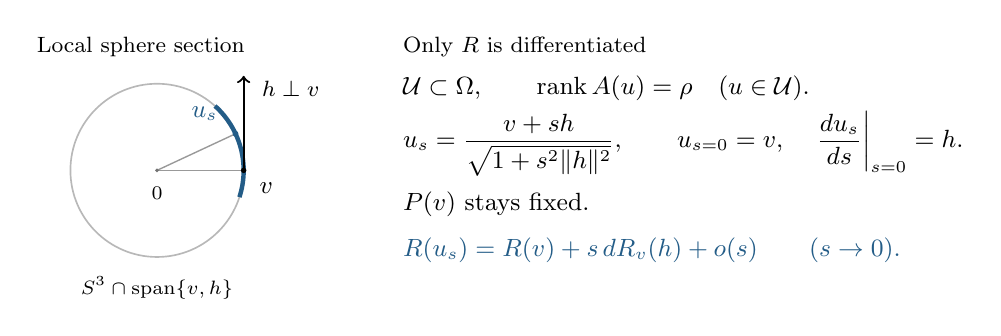
\begin{tikzpicture}[x=1cm,y=1cm,font=\small]
  \definecolor{tangentblue}{RGB}{35,92,135}

  \node[anchor=west,font=\footnotesize] at (0,3.02)
    {Local sphere section};
  \coordinate (O) at (1.65,1.45);
  \coordinate (V) at (2.75,1.45);
  \coordinate (Us) at (2.6469,1.9149); %
  \draw[black!28,line width=0.6pt] (O) circle[radius=1.1];

  \draw[tangentblue,line width=1.6pt]
    (2.6962,1.1101) arc[start angle=-18,end angle=48,radius=1.1];
  \draw[black!40,line width=0.5pt] (O) -- (V);
  \draw[black!40,line width=0.5pt] (O) -- (Us);
  \fill[black!55] (O) circle[radius=0.025];
  \node[anchor=north,font=\scriptsize] at (1.65,1.36) {$0$};

  \draw[->,line width=0.8pt] (V) -- (2.75,2.65);
  \node[anchor=west,font=\footnotesize] at (2.86,2.49) {$h\perp v$};
  \fill (V) circle[radius=0.035];
  \node[anchor=north west] at (2.83,1.42) {$v$};
  \fill[tangentblue] (Us) circle[radius=0.037];
  \node[anchor=south east,text=tangentblue] at (2.54,1.96) {$u_s$};
  \node[anchor=north,font=\scriptsize] at (1.65,0.22)
    {$S^3\cap\operatorname{span}\{v,h\}$};

  \node[anchor=west,font=\footnotesize] at (4.65,3.02)
    {Only $R$ is differentiated};
  \node[anchor=west] at (4.65,2.49)
    {$\mathcal U\subset\Omega,\qquad \operatorname{rank}A(u)=\rho\quad(u\in\mathcal U).$};
  \node[anchor=west] at (4.65,1.79)
    {$\displaystyle u_s=\frac{v+sh}{\sqrt{1+s^2\|h\|^2}},
      \qquad u_{s=0}=v,\quad \left.\frac{du_s}{ds}\right|_{s=0}=h.$};
  \node[anchor=west] at (4.65,1.02)
    {$P(v)\text{ stays fixed.}$};
  \node[anchor=west,text=tangentblue] at (4.65,0.43)
    {$R(u_s)=R(v)+s\,dR_v(h)+o(s)\qquad(s\to0).$};
\end{tikzpicture}
\caption{A schematic local tangent step, for a fixed nonzero $h\in v^\perp$.
The highlighted arc lies in a chosen constant-rank neighborhood $\mathcal U$;
the expansion of $R$ is used only for small $s$ with $u_s\in\mathcal U$.
The pictured section belongs to the parameter sphere, whereas $P(v)$
and $R(u_s)$ act on the separate block spaces $\mathbb R^a$ and
$\mathbb R^c$.}
\label{fig:local-tangent}
\end{figure}


The linear map \(J:v^\perp\to\R^3\) is an isomorphism. Indeed, if
\(Jh=0\), then \(v_0\ne0\) gives
\(h=(h_0/v_0)v\); since \(h\perp v\), this forces \(h=0\).
Both spaces have dimension three.
Consequently the matrix
\[
 F(z,y)=P(v)B(y)dR_v(J^{-1}z),\qquad z,y\in\R^3,
\]
has entries that are bilinear in \(z,y\), since \(B\) and the differential
\(dR_v\) are linear. In fixed orthonormal bases,
each entry \(\ell_{ij}(z,y)\) satisfies
\[
 \ell_{ij}(z,y)^2
 \le \norm{F(z,y)}_{\op}^{2}
 =b(z,y)
 \qquad(z,y\in\R^3).
\]
Lemma~\ref{lem:form} forces every entry to vanish identically.
Equation~\eqref{eq:tangent-identity} would therefore make \(b\)
identically zero, contradicting \(b(e_1,e_1)=1\).
This excludes the hypothetical finite pencil and completes the proof.
\end{proof}

\section{Removing a determinant factor}\label{sec:reduced}

The polynomial $p$ makes the positive-map construction explicit through
a $4\times4$ determinant. We now remove a factor that is unnecessary for
its hyperbolicity cone. A larger block determinant shows directly that
the quotient remains polynomial at singular $X$.

\begin{proof}[Proof of Corollary~\ref{cor:reduced}]
For the standard coordinate vectors $e_i$ of $\R^3$, put
\[
 K_i=\begin{pmatrix}0&e_i^\top\\-e_i&0\end{pmatrix}\in\R^{4\times4},
 \qquad C=\begin{pmatrix}K_1&K_2&K_3\end{pmatrix}\in\R^{4\times12}.
\]
Here $U\otimes V$ denotes the block matrix with blocks $U_{ij}V$.
Direct block multiplication in~\eqref{eq:phi} gives, for $T\in\Sym^4$,
\[
 \Phi_y(T)=\sum_{i,j=1}^3 Q(y)_{ij}K_iTK_j^\top
          =C\bigl(Q(y)\otimes T\bigr)C^\top.
\]
Define the polynomial
\begin{equation}\label{eq:reduced-polynomial}
 q(X,Z,y)=\det\begin{pmatrix}
 I_3\otimes X&C^\top\\
 C\bigl(Q(y)\otimes I_4\bigr)&Z
 \end{pmatrix}.
\end{equation}
For invertible $X$, taking a Schur complement yields
\[
 q(X,Z,y)=(\det X)^3\det\bigl(Z-\Phi_y(X^{-1})\bigr).
\]
Comparison with~\eqref{eq:inverse-formula} proves the polynomial identity
\begin{equation}\label{eq:reduced-factor}
 p(X,Z,y)=(\det X)q(X,Z,y)
\end{equation}
first for invertible $X$ and then everywhere by continuity.
Since $p$ and $\det X$ are homogeneous of degrees $20$ and $4$, this
identity makes $q$ homogeneous of degree $16$; also $q(e)=1$.
For each real $(X,Z,y)$, the polynomial $q(te-(X,Z,y))$ is a factor of
the real-rooted polynomial $p(te-(X,Z,y))$. Hence $q$ is hyperbolic
with respect to $e$.

Write $K_q=\Lambda_+(q,e)$. The factorization~\eqref{eq:reduced-factor}
gives
\begin{equation}\label{eq:cone-intersection}
 K=\{(X,Z,y):X\succeq0\}\cap K_q,
\end{equation}
because the roots contributed by $\det(tI_4-X)$ are the eigenvalues of
$X$. It remains to show that $K_q$ already forces $X\succeq0$.
The polynomial $q$ is even in $y$, so $(X,Z,y)\in K_q$ implies
$(X,Z,-y)\in K_q$. By convexity of hyperbolicity
cones~\cite{garding-1959}, their midpoint $(X,Z,0)$ also belongs to $K_q$.
But~\eqref{eq:reduced-polynomial} gives
\[
 q(X,Z,0)=(\det X)^3\det Z,
\]
whose closed hyperbolicity cone in this slice is exactly
$\{(X,Z,0):X\succeq0,\ Z\succeq0\}$.
Thus $X\succeq0$ throughout $K_q$, and~\eqref{eq:cone-intersection}
implies $K_q=K$. Theorem~\ref{thm:main} now supplies nonspectrahedrality.
\end{proof}

\appendix
\section{A path-containment assertion}
\label{app:opposition}

Theorem~53 (pp.~16--17) of version~1 of Gonz\'alez Nevado's
\cite{gonzalez-nevado-2026} states a positive solution of the geometric
Generalized Lax conjecture. Its proof invokes Theorem~52 (p.~16), which asserts
containment of a fixed rigidly convex set throughout a smooth real-zero
deformation from a product of normalized tangent linear factors to a
multiple of the defining polynomial. The following example violates
that intermediate assertion under its stated hypotheses.

A real polynomial $g$ with $g(0)=1$ is \emph{real-zero} if the roots of
$s\mapsto g(sx)$ are real for every real vector $x$. Its closed
rigidly convex set is the closure of the component of $\{g\ne0\}$
containing the origin. Fix $a,b,\eta>0$ and, in one variable, put
\[
 g(x)=(1-x/a)(1+x/b),\qquad
 c(t)=1+\eta\sin^2(\pi t),\qquad
 H_t(x)=g(c(t)x),\quad 0\le t\le1.
\]
The zero set of $g$ is the compact smooth set $\{-b,a\}$.
The normalized tangent linear factors at these two points are
$1+x/b$ and $1-x/a$, whose product is $g$. Every $H_t$ has value $1$
at the origin and two distinct real roots,
\[
 -\frac{b}{c(t)}\quad\hbox{and}\quad\frac{a}{c(t)}.
\]
Thus the path depends smoothly on $t$ and consists of real-zero
polynomials with compact smooth zero sets. It even admits the smooth
monic real symmetric determinantal representation
\[
 H_t(x)=\det\begin{pmatrix}
 1-c(t)x/a&0\\
 0&1+c(t)x/b
 \end{pmatrix}.
\]
Both endpoints equal $g$, so the final polynomial is $g$ times the
constant cofactor $1$, as allowed by the stated hypotheses.
Nevertheless the rigidly convex set of $H_t$ is
\[
 \left[-\frac{b}{c(t)},\frac{a}{c(t)}\right],
\]
which is strictly smaller than $[-b,a]$ whenever $0<t<1$.
Consequently it does not contain the rigidly convex set of $g$.

The parameters $a,b>0$ describe the open family of normalized real
quadratics with negative leading coefficient, so the failure is not
confined to a symmetric or multiple-root example. The parameter $\eta$
may be arbitrarily small. The cited Theorem~52 states no restriction
to two or more variables, no lower bound on pencil size, and no
requirement that the endpoint cofactor be nonconstant.

This example refutes the all-intermediate-times conclusion of that
theorem. Its endpoints coincide, so it does not refute an endpoint-only
statement. The nonspectrahedrality result of this paper follows from
the construction and obstruction proved above.

\bibliographystyle{plainnat}
\bibliography{references}
\end{document}
